\section{Introduction}
\label{sec:intro}

Vision-Language Models (VLMs)~\cite{li2024llava,liu2023llava} have emerged as a cornerstone of multimodal AI, enabling joint reasoning over visual and textual data. 
By integrating advances from computer vision and natural language processing, VLMs excel at tasks such as video captioning~\cite{yang2023vid2seq,zhang2024video}, visual question answering~\cite{sinha2024guiding_vlm_sel_for_vqa,das2025vlm_continual_vqa}, and cross-modal retrieval~\cite{li2022blip}. 
Following a similar trajectory to Large Language Models (LLMs)~\cite{brown2020language, devlin2018bert}, modern VLMs have rapidly scaled in size and data, resulting in notable accuracy gains. 
However, this scaling significantly increases compute and memory demands, posing challenges for deployment, especially on edge devices~\cite{sharshar2025vision}.

Fortunately, video-based inputs offer a key opportunity: high visual redundancy~\cite{dynamicllava,voco,prumerge,fastv,wang2025corematching}.  
As shown in \Fig{fig:intro}(a), adjacent frames often share similar backgrounds and foreground objects.  
Since VLMs tokenize each frame independently~\cite{li2024llava,zhang2024video}, many tokens across or within frames are redundant.  
This has motivated techniques such as token pruning~\cite{sah2024token_pruning_vit,wang2025corematching} and token merging~\cite{bolya2023token} to reduce computation.  
However, most prior work focuses on algorithmic strategies without considering hardware alignment.  
For instance, Token Merging~\cite{bolya2023token} introduces a ToMe module that increases runtime by up to 36.8\%~\cite{yoo2024adaptiv}.

Recent designs such as AdapTiV~\cite{yoo2024adaptiv} and CMC~\cite{song2024cmc} address these inefficiencies at the hardware level.  
AdapTiV implements a simplified ToMe module in hardware, while CMC leverages video-codec-inspired compression (e.g., H.264~\cite{wiegand2003overview}) via an external codec block.
However, both approaches largely translate existing algorithms without embracing full hardware-{algorithm} co-design. 
First, both {targeted for Vision Transformers (ViTs)~\cite{dosovitskiy2020image}, }focus only on visual redundancy and overlook the cross-modal nature of VLMs. 
CMC’s codec ignores language inputs, and AdapTiV only supports static images, missing video-language interactions.
Second, both operate at global token-level granularity, which is inefficient for both algorithm and hardware due to high overhead and poor locality.
To enable efficient VLM deployment, a more holistic co-design approach is needed, one that leverages cross-modal redundancy while aligning with hardware-friendly processing granularity.

In this study, we propose a novel architecture, \textbf{\proj{}}, to accelerate VLM inference by performing \textbf{\textit{streaming concentration}}, a multilevel compression technique that removes visual and cross-modal redundancy in a streaming-friendly, on-chip processing fashion.

From the \textbf{algorithmic perspective}, \proj{} performs redundancy concentration at three levels of granularity.  
First, it leverages semantic understanding to retain only visual regions relevant to the textual prompt.  
Prior work~\cite{rao2021dynamicvit,bolya2023token,song2024cmc,yoo2024adaptiv} relies on static metrics like token magnitude, which fail to capture prompt-conditioned semantics in VLMs.  
As shown in \Fig{fig:intro}(a), attention may shift from a foreground object (e.g., a dog) to a background element (e.g., a flower), depending on the question (see details in \Sec{subsec:motivation_algo}).
To address this, \proj{} introduces a prompt-aware importance analyzer that dynamically prunes visual tokens based on cross-modal attention, improving both accuracy and efficiency.

Second, as illustrated in \Fig{fig:intro}(b), \proj{} groups retained tokens into spatiotemporal blocks, using the last token (e.g., token~$h$) as the key for localized similarity comparisons. 
The key token is compared with others in its block. 
This is applied across the video, treating each token in turn as a key. 
This technique resembles a 3D convolutional sweep that progressively concentrates similarity through localized matching. 
By operating within small spatial-temporal windows, \proj{} avoids global comparisons, making the process compute-efficient and highly streamable.

Third, \proj{} explores redundancy at the vector level. 
Due to video motion, a token may align with multiple shifted tokens in adjacent frames. 
As shown in \Fig{fig:intro}(c), token $h$ may share features with parts of tokens $c$ and $d$. 
Relying on a single best-matched token may lose information. 
Instead, \proj{} performs vector-wise comparisons, allowing each vector to match multiple candidates and capture richer sub-token similarity. 
By integrating these three levels, \proj{} achieves up to \textbf{83\%} (\textbf{80\%} on average) computational sparsity through multilevel concentration, significantly outperforming CMC and AdapTiV, which typically reach only 40--50\%, under similar accuracy.

\begin{figure}
    \centering
    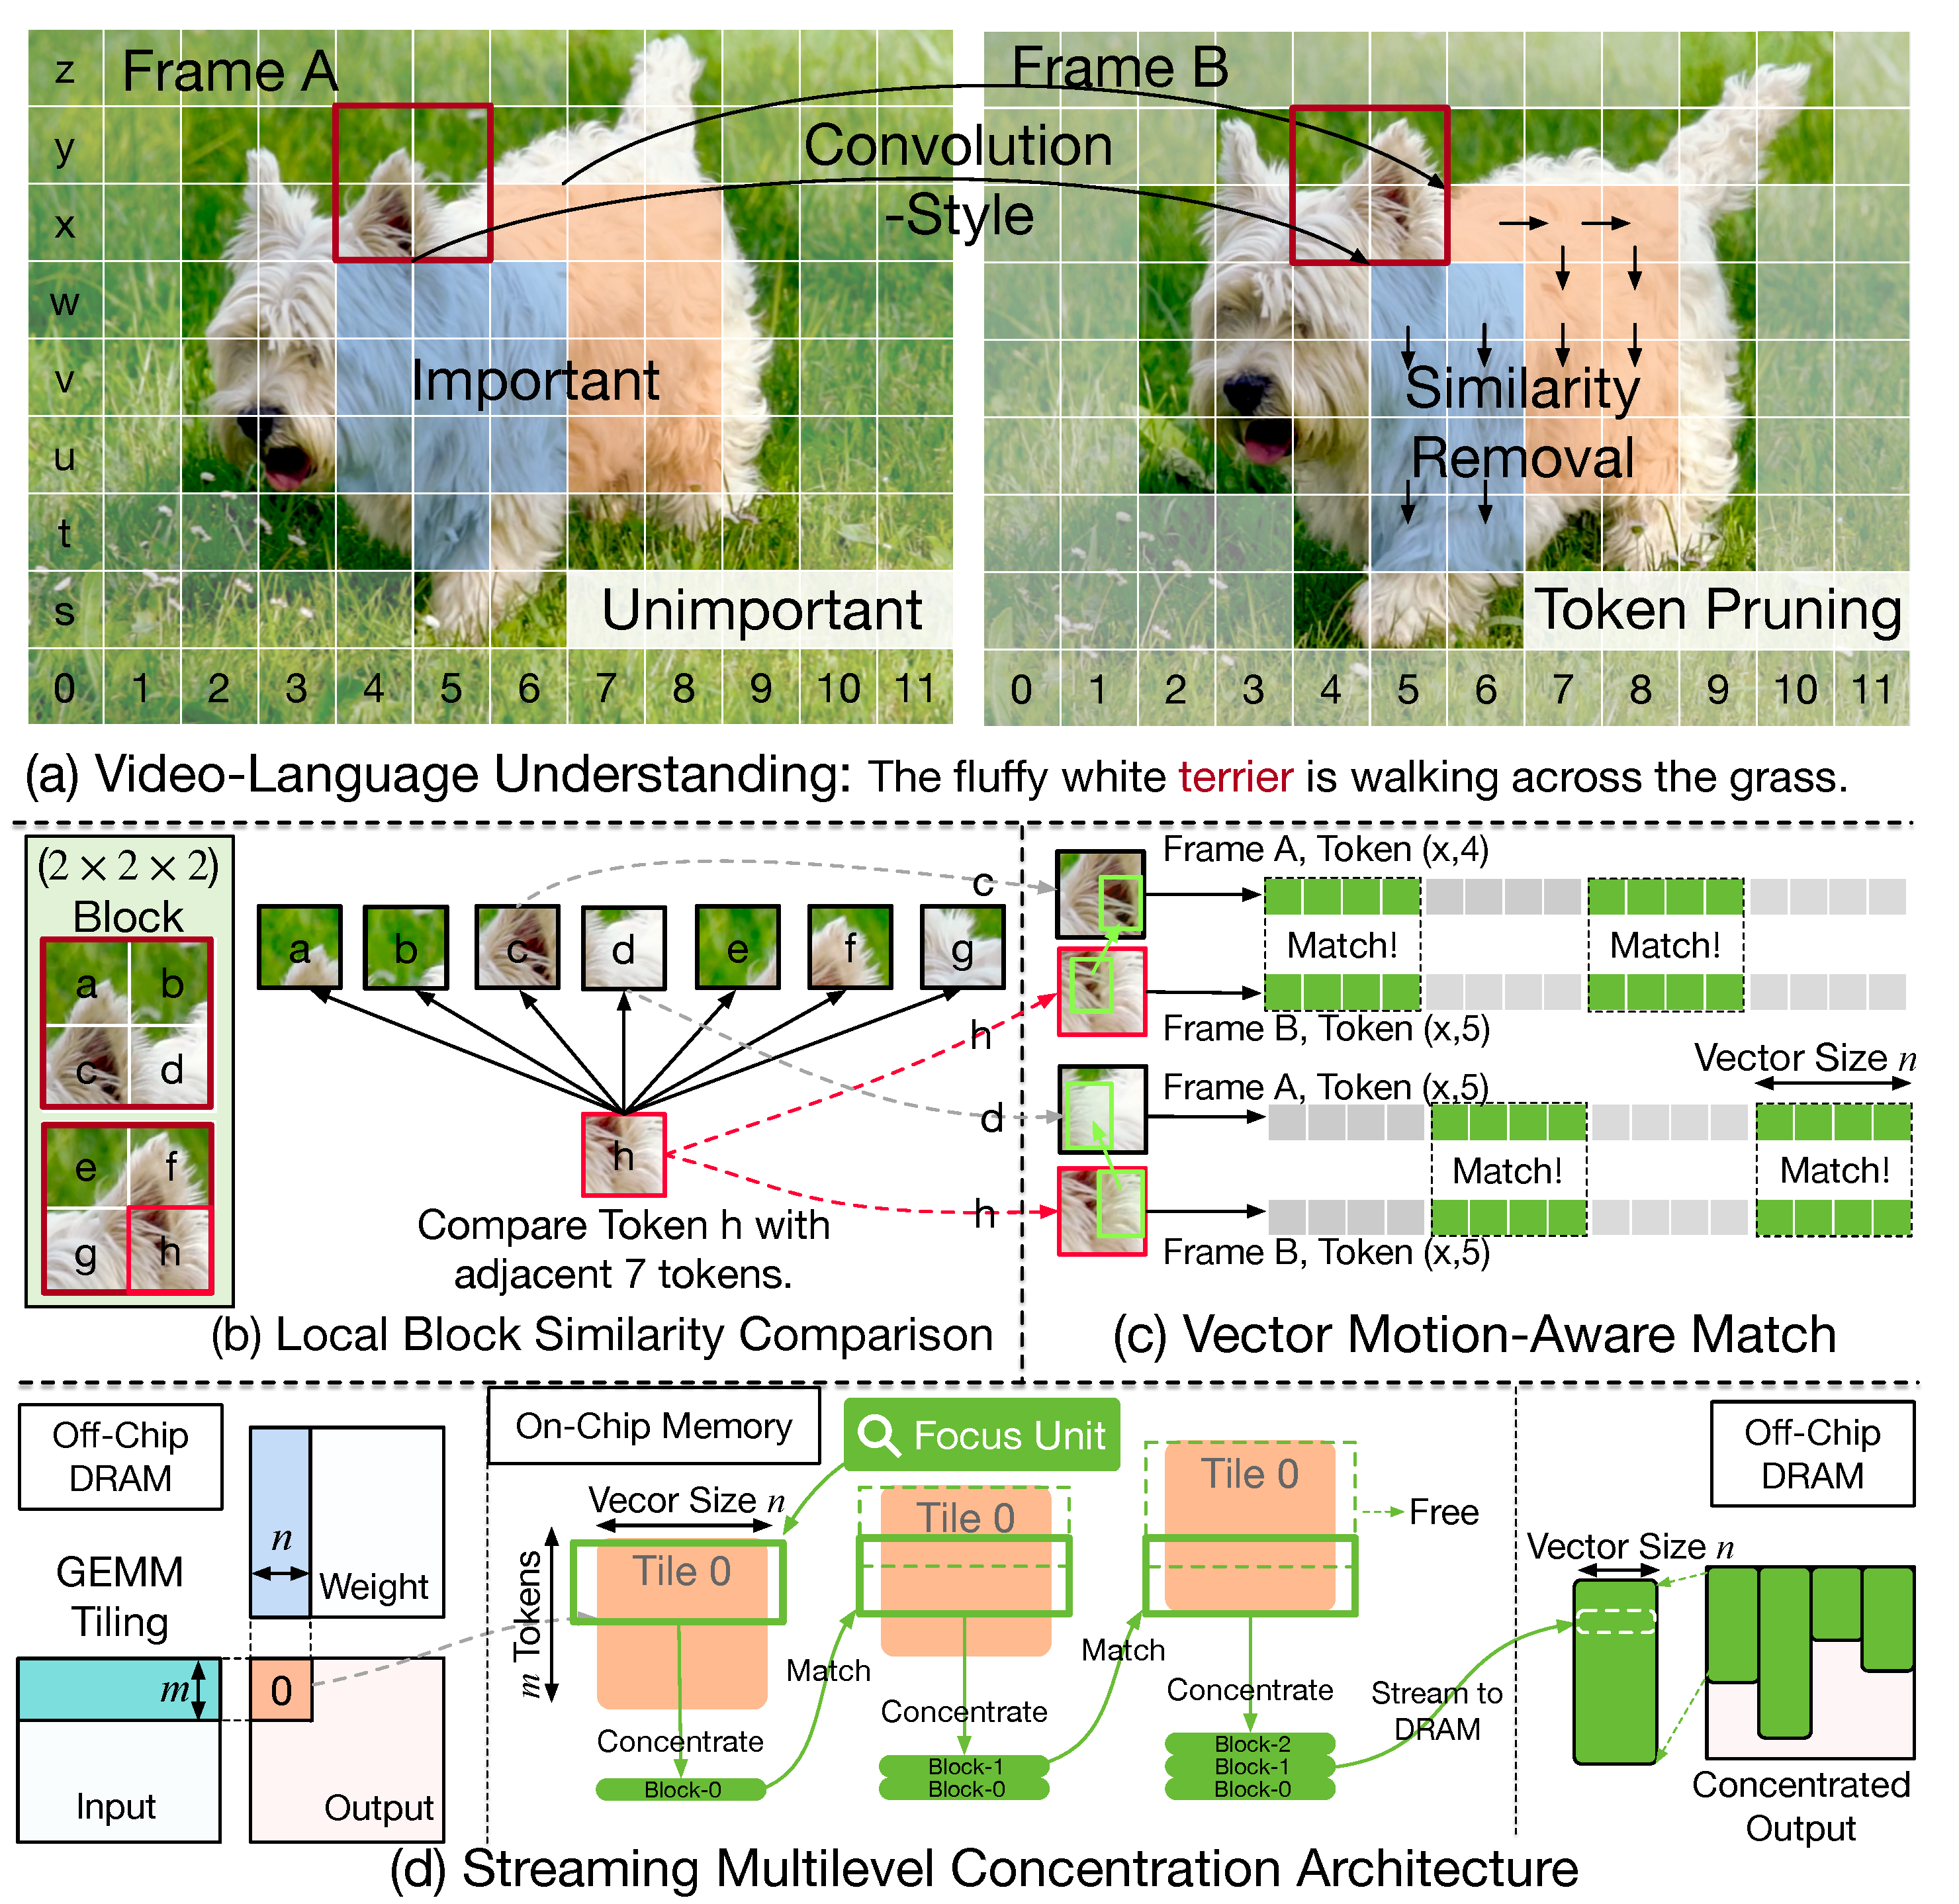
\includegraphics[width=1\linewidth]{figure/intro.pdf}
    % \vspace{-6mm}
    \caption{Overview of the streaming multilevel concentration architecture.}
    \label{fig:intro}
    % \vspace{-5mm}
\end{figure}

From the \textbf{architectural perspective}, \proj{} is designed to efficiently support multilevel concentration through tight alignment with General Matrix Multiplication (GEMM) tiling.  
As shown in \Fig{fig:intro}(d), its vector- and block-level operations naturally align with the tiling strategies widely adopted in systolic-array–based accelerators such as TPUs~\cite{jouppi2023tpuv4} and GPUs~\cite{choquette2021nvidia}.
GEMM tiling addresses on-chip memory constraints by dividing matrices into small, independently processed tiles. 
Each tile is handled by the PE array in isolation, enabling efficient, in-place \textbf{vector-level} similarity detection and compression.
By eliminating redundancy locally within each tile, \proj{} minimizes data movement and reduces both compute cost and DRAM traffic. 
In contrast to global token-wise methods that rely on costly off-chip access, \proj{} achieves fine-grained, on-chip processing in a hardware-efficient manner.


At the \textbf{block level}, \proj{} draws inspiration from CNN accelerators~\cite{chen2016eyeriss,du2015shidiannao}, using a sliding window to stream and process output tokens directly from the compute core (e.g., systolic array), maximizing locality and sustaining high throughput. 
To handle the non-contiguous nature of VLM tokens within a block, we adopt a convolution-style layout that preserves streaming flow while ensuring alignment for block-wise matching.
At the {semantic-level, which corresponds to the \textbf{token level}}, \proj{} integrates into the attention layer to identify and retain the most relevant tokens based on cross-modal attention scores.  
Through dedicated scheduling, it performs token selection in a streaming fashion, enabling compression prior to memory write-back without stalling GEMM execution.

\proj{} operates as a standalone module, similar to pooling or activation, without interfering with the core computation pipeline.  
Its modularity enables broad applicability and scalability while maintaining high compression efficiency.  
By co-optimizing the algorithm and architecture, \proj{} achieves up to \textbf{5.0$\times$} reduction in computation and \textbf{4.5$\times$} reduction in memory footprint for VLM inference.
Occupying only {\textbf{2.7\%}} of the systolic array area, it is lightweight and well-suited for edge deployment.
{Our contributions are as follows:}
\begin{itemize}
    \item We propose {multilevel concentration}, a hardware-oriented redundancy removal paradigm that eliminates semantic-, block-, and vector-level redundancy in VLMs.

    \item We develop a co-designed {streaming concentration architecture} that aligns with tiling-based execution and memory access patterns with minimal hardware overhead.

    \item To the best of our knowledge, \proj is the first architecture tailored for VLMs, delivering {2.60$\times$}/{2.35$\times$} performance and {{2.98$\times$}/{3.29$\times$}} energy efficiency gains over AdapTiV and CMC, respectively.
\end{itemize}
